\documentclass{sbthesis}
\usepackage{graphicx}

% \IncludeFig{caption}{label}{file}{scale}
\newcommand{\IncludeFig}[4]{
\begin{figure}[h]
\centering
\includegraphics[scale=#4]{#3}
\caption{#1}
\label{#2}
\end{figure}
}

\title{Isocenter Localization In MRI Imaging System with GPGPU}
\author{Zongqi Cai}
\Department
\EmailAddress{caiz@csusb.edu}
\Advisor{Keith Evan Schubert}
\Committee*{Kay Zemoudeh}{Haiyan Qiao}{}
\CSUSBDate{Janurary 2010}
\Copyright

%\AbstractText{}
%\AcknowledgementText{}
%\DedicationText{To Zel and Septimus.}
\NoTables
\NoFigures

\begin{document}
\ThesisProposal
\Chapter{Introduction}
\label{Introduction}

\indent

Magnetic Resonance Imaging (MRI) is a medical imaging technique to visualize detailed
internal structures and limited function of body. It provides much greater contrast
between the different soft tissues of the body than computed tomography (CT), making
MRI especially useful in neurological (brain), musculoskeletal, cardiovascular, and
oncological (cancer) imaging. However, the geometric distortion in modern MR scanners can
greatly reduce the accuracy of images. The most prominent source of distortion
comes from the nonlinearity of the magnetic field used to produce the images.
Several MRI distortion correction methods have been described in various literatures,
which are usually based on scanning a phantom cube (fig \ref{fig:1}) with accurately known reference structures \cite{R3, R4, R5, R6}. However, they either cannot provide high level of geometric
accuracy required to confidently perform high-precision functional radiosurgery, e.g. brain
tagets, or cannot perform the correction process in a tolerable time frame for clinical use \cite{tom}.
Most of these works calculate the distortion based on an inaccurate assumption of the location of the isocenter
of the magnetic field.
In this work, a different approach is proposed that uses the isocenter as one of the unknown factors and calculates
both distortion parameters and the isocenter location.  %, which has never been done before. -- I would either leave this out, or show more proof of this claim
This work will use an efficient implementation of this
method using General-Purpose Computing on Graphics Processing Units (GPGPU).

\begin{figure}[htb]
  \begin{minipage}{0.80\linewidth}
    \centering
    \centerline{\mbox{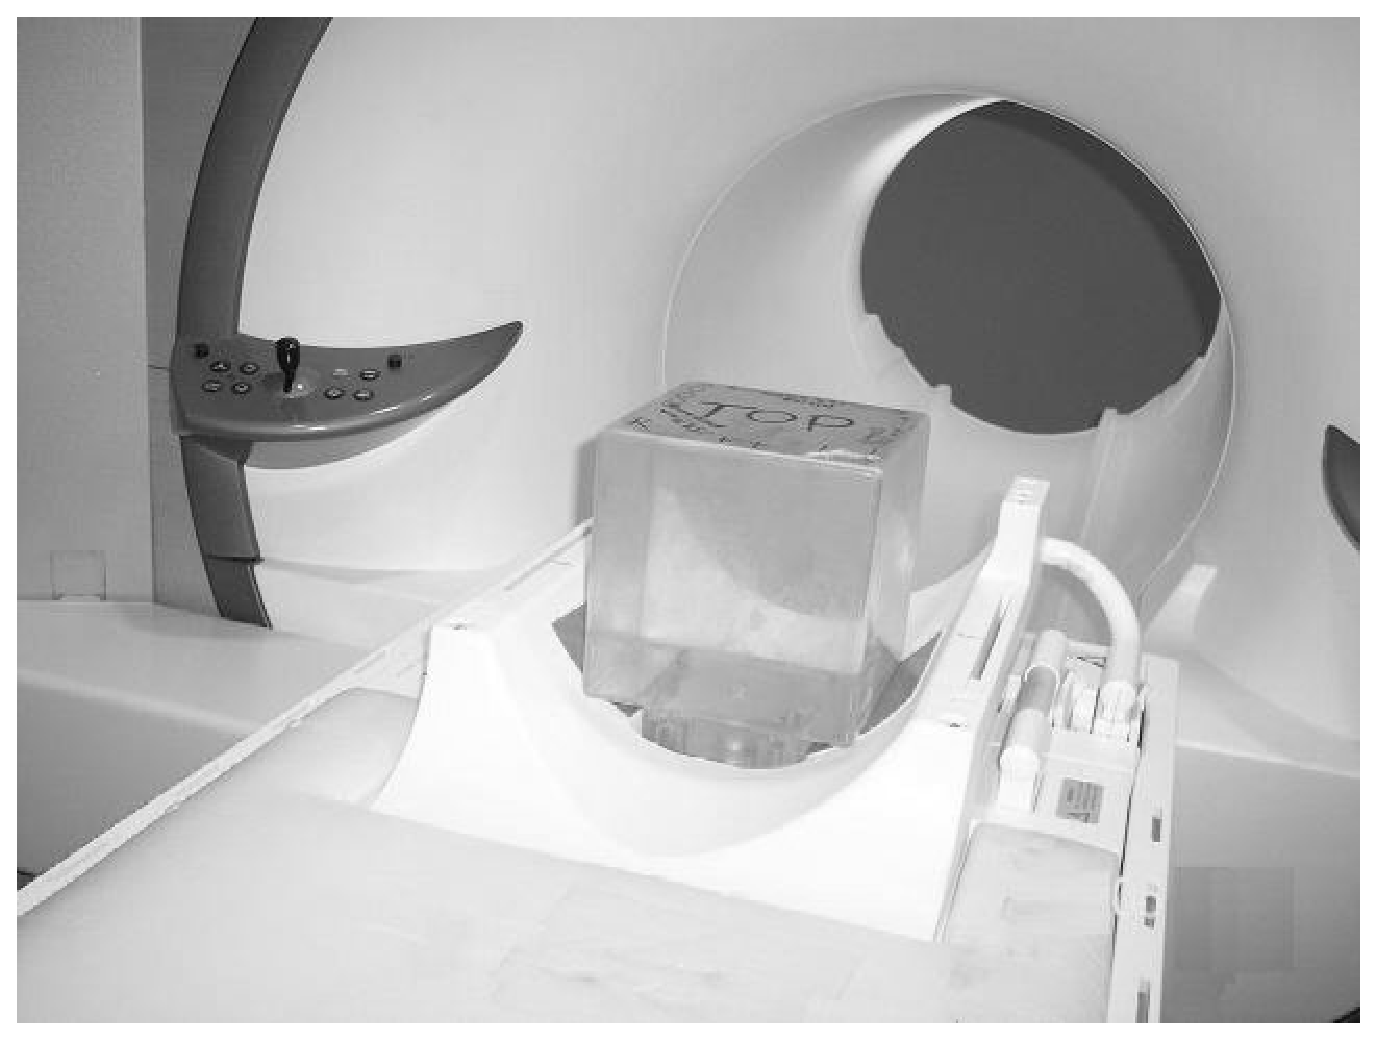
\includegraphics[width=4in]{images/phantom_scanner2.eps}}}
%    \centerline{New device}\medskip
    \centerline{}\medskip
  \end{minipage}
  \caption{A phantom cube made of plexiglas and filled with oil is ready for scanning} \label{fig:1}
\end{figure} 


\section{Background}

The clinical application of protons was first suggested over 60 years ago \cite{Wil46}.
The ability to penetrate human tissue, delivering high dosage of proton beams at a target
region and being able to concentrate on a very small target area make protons ideal for use in noninvasive surgery \cite{Wil46}. Currently, Loma Linda University
Medical Center (LLUMC) is using proton beams to treat patients with tumors or
vascular malformations in the brain.
Due to the effectiveness of proton radiosurgery, a new system is proposed to treat
even smaller targets, more specifically, cranial targets.  However, this requires higher
accuracy of the treatment system. The current system can treat targets as small as 1 to 3 cm.  Target localization is accomplished using CT and projection angiography.
In order to achieve higher accuracy, MRI is to be used for target localization in the new
system. The major obstacle of using MRI is the gradient nonlinear
distortion on MRI images caused by the magnetic field of the scanner.
Two of the most important requirements for a successful distortion correction are:

\begin{enumerate}
\item The distortion correction must have submillimeter accuracy.
\item The correction process must be finished within 15 minutes.
\end{enumerate}

% I added some more detail in this paragraph

%The iteracy that this work is based on presented gradient nonlinearity correction method based on a cubic phantom MRI data set\cite{tom}.
This work is based on a published method for gradient nonlinearity correction using a cubic phantom MRI data set \cite{tom}. The published method utilizes the sum of spherical
harmonics to model the geometrically warped planes of the cube, and applies the model
to correct arbitrary image sets acquired with the same scanner. The cube is
placed in the MRI scanner such that the cube's center is exactly in the center of the MRI scanner.  This work assumes the center of the MRI scanner corresponds to the isocenter of the
magnetic field of the scanner. Opposite faces of the phantom are averaged, and three midplanes are fit to these surfaces.  Due to the symmetric property of the magnetic field,
the midplanes of different orientations of the phantom cube are undistorted.  Through each midplane, the ideal planes of different surfaces
of the cube are calculated simply by shifting the midplane to the direction
of the ideal plane by one-half the length of the cube. For each pixel on
the ideal plane, the sum of spherical
harmonics equation \ref{eq:spherical_harmonics} is applied to transform that pixel to the corresponding location on the distorted plane.

\begin{equation} \label{eq:spherical_harmonics}
\bar{\alpha} = \alpha(1 + K_{\alpha_0}(x^2 + y^2) + K_{\alpha_1}z^2 +
K_{\alpha_2}z^2(x^2 + y^2) + K_{\alpha_3}(x^2 + y^2)^2 +
K_{\alpha_4}z^4)
\end{equation}

Where $\bar{\alpha}$ and $\alpha$ are undistorted and distorted 3D coordinate respectively; $x$, $y$ and $z$ are coordinates of $\alpha$ on each axis; $K_{\alpha_i}$ are distortion parameters. Thus the distortion parameters in
equation \ref{eq:spherical_harmonics} are computed using linear least squares
technique.

Several assumptions are made for this model:
\begin{itemize}
  \item The phantom is (reasonably) centered with respect to the gradient isocenter of the scanner.
  \item The distortion is (reasonably) symmetric for each pair of faces.
  \item The origin of the DICOM patient coordinate system represents the position of the gradient isocenter.
\end{itemize}

However, positioning the phantom with respect to gradient isocenter is very difficult,
making it nearly impossible to perfectly center the phantom. After performing numerous
scans by Permedics Inc and LLUMC over the past several years, the issue of phantom centering has been identified
as a crucial factor in the quality of image data.  Improper centering of the phantom
in the scanner produces strong asymmetry in the phantom surfaces, thereby affecting the
accuracy of the distortion correction.  Therefore, the assumption that the distortion
is symmetric for each pair of phantom faces is invalid.

The assumption that the origin of the DICOM patient coordinate system corresponds to the isocenter of the magnetic field in the MRI scanner is also invalid. Siemens
engineers have confirmed that the true location of the gradient isocenter is unknown.
Investigating this further appeared to confirm this claim:  every scan performed thus far features a -10mm offset in Y in order to center the field of view on the phantom.  Therefore, the DICOM origin is shifted -10mm in $Y$ for each image.  But, the distortion inherent to each pair of phantom surfaces appears to be quite symmetric.  If the gradient isocenter was truly located at the DICOM origin, then the images would be expected to contain significant asymmetry in the distortion.  This is not the case in recent phantom studies.

In addition, the computation, including image filtering, distortion parameters
computation and final correction, average takes about 20-30 minutes.  In some cases, the calculation
could require as much as 40 minutes. This is far from the ideal 15 minutes requirement for clinical use.

\section{Significance}

% Which equation are you referring to here?  It would be better to reference the equation, instead of saying "the equation above"

Consider the minimization of the original expression for the sum of spherical harmonics:

\begin{equation} \label{eq:spherical_harmonics_2}
0 = \alpha(1 + K_{\alpha_0}(x^2_i + y^2_i) + K_{\alpha_1}z^2_i +
K_{\alpha_2}z^2_i(x^2_i + y^2_i) + K_{\alpha_3}(x^2_i + y^2_i)^2 +
K_{\alpha_4}z^4_i)
\end{equation}

The correction method this work proposes is on a pixel-to-pixel basis instead of a plane to plane basis.
Consider a point $P$ = $[X,Y,Z]$, where $X$, $Y$, and $Z$ are represented in equation \ref{eq:spherical_harmonics_2}. Each $X$, $Y$, and $Z$ describes the distance of $P$ from the DICOM origin (gradient isocenter), previously assumed to be at [0,0,0].  Past MRI studies have confirmed that the gradient isocenter is not at [0,0,0], therefore it is necessary to shift the DICOM origin appropriately by some offset $[\delta,\beta,\gamma]$.  Shifting the DICOM origin by this amount yields the new expression for $P$:

\begin{eqnarray}
P = [X - \delta, Y - \beta, Z - \gamma]
\end{eqnarray}

Substitute the new expression for $P$ into the sum of spherical harmonics expression:

$$0 = \alpha(1 + K_{\alpha_0}((x_i - \delta)^2 + (y_i - \beta)^2)$$
$$+ K_{\alpha_1}(z_i - \gamma)^2 + K_{\alpha_2}(z_i - \gamma)^2((x_i - \delta)^2 + (y_i - \beta)^2)$$
$$+ K_{\alpha_3}((x_i - \delta)^2 + (y_i - \beta)^2)^2 + K_{\alpha_4}(z_i - \gamma)^4)$$

Therefore, by expressing $P$ in this manner, the position of the true gradient isocenter becomes
$[\delta, \beta, \gamma]$. To solve for $\delta$, $\beta$, $\gamma$ and $K_{\alpha}$, we do not need
to have a full plane, as long as enough data points exist, and each data point exhibits a significant amount of distortion. The system can be solved using a linear least squares technique.

To collect the data sets, a new phantom (Fig \ref{fig:2}), is proposed to capture data points on only the corner sections
of the original phantom cube.  Since these sections are located far away from the gradient isocenter, they will exhibit the largest amount
of distortion when compared to other sections closer to the gradient isocenter. The image slices that
would be used are those close to each surface of the phantom. For each of these images a 
filtering process will be applied to obtain only data points on the edge of phantom cube. 

\begin{figure}[htb]
  \begin{minipage}{0.80\linewidth}
    \centering
    \centerline{\mbox{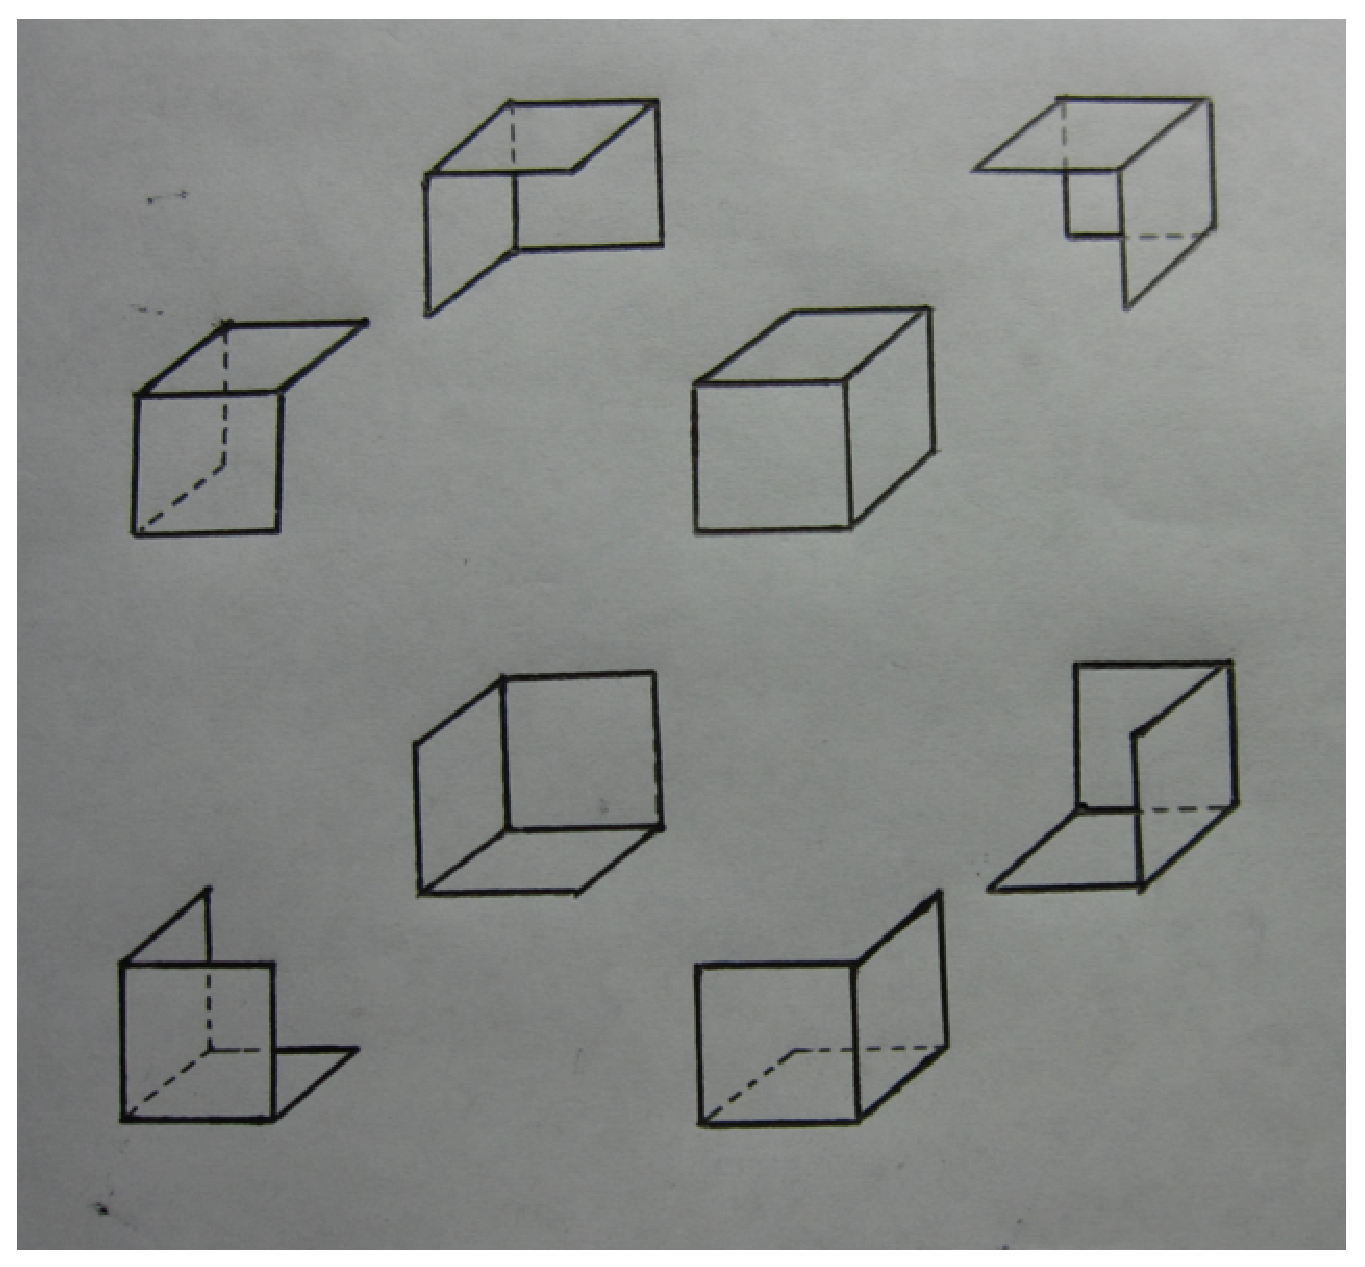
\includegraphics[width=4in]{images/model2.eps}}}
%    \centerline{New device}\medskip
    \centerline{}\medskip
  \end{minipage}
  \caption{The new phantom, designed to collect data at the corners of the MRI scan.}  \label{fig:2}
\end{figure}

The reason for constructing a new phantom is that a phantom cube larger than original size (159.50 mm x 159.70 mm x 158.11 mm) is needed to 
capture the distortion of larger MRI scanner while the manufacturer who produced the original
phantom cube was having difficulty produce an accurate cubic phantom larger than the
one shown in \ref{fig:1}. The eight parts, shown in fig \ref{fig:2}, will be interconnected and placed inside a water tank for scanning.
For each image, eight curves representing the intersection between the surface of the material
and water will be obtained, and will be used for calculating the gradient nonlinearity distortion correction.

All the procedures involved, including image filtering and linear least square calculations, would be implemented on a system running a NVIDIA GTX 280 graphics card. This series of Graphics Processing Units (GPUs)
contains 240 processing cores each operating at
1296Mhz \cite{GTX280}. They can be programmed using a subset of
the C programming language called CUDA (Compute Unified Device Architecture). Because the
GPUs are accessed via a PCI Express (PCIe) x16 2.0 bus, they can handle a data throughput of
8.0 GB/s (500MB/s * 16 PCIe lanes). The
PCIe bus will be a bottleneck because memory bandwidth on
the motherboard, as well as the GPU, are much higher than 8.0 GB/s. Due to this
bottleneck, algorithms need to be designed to maximize the number of
calculations per data transfer.

\Chapter{Research Execution Plan}

% I reworded pieces of this section to remove personal pronouns (e.g., "I")

%I will spend Winter and Spring 2010 to do my research and writing my thesis. In about three weeks,
%the construction of new device shown in figure \label{fig:2} will be started. In about another
%4-5 weeks, the device should be availabe for testing. Mean time, I will be developing parallel
%algorithms, including edge detector, QR least squares, etc, that are required for testing. All
%programs eventually should be written in C/C++ and run on CUDA capable Graphics Card, and
%matlab will be used for testing purpose.
%When the construction is finished, my algorithms should be ready for testing.
%At this point, I will compile my research into a partial draft (Deliverable 1).
%For the next 3-4 weeks, I will perform series of tests and adjustment on my code, compile
%my test data and finish my first rough draft (Deliverables 2 and 3).
%The rest of the time will be use to compile my thesis and prepare for its defense. (Deliverables 4, 5 and 6).

The research and work for this project will be performed during Winter and Spring 2010. First,
construction of the new phantom shown in figure \ref{fig:2} will commence. Next the phantom is constructed to be available for scanning and data gathering. While the phantom is constructed and prepared for scanning, development of the parallel algorithms will begin.  The parallel algorithms that will be developed include an edge detection algorithm and QR factorization (for linear least squares). All programs will be written in C/C++ and executed on the CUDA-capable GPU.  Additionally, MATLAB will be utilized for testing purposes to confirm the accuracy of the C/C++ and CUDA algorithms.  Software development is expected to be complete by the time the phantom is available for scanning and testing.

The following deliverables will be produced:

\begin{itemize}
  \item Once software development is complete, the status of the research will be compiled into a scientific paper, which will serve as an early thesis draft.
  \item Software will be verified for accuracy and any necessary adjustments will be made to the code. Qualitative and quantitative results will be gathered.
  \item All new details of the research, as well as results gathered from testing, will be added to the thesis draft.
  \item With all data gathered, the thesis draft will be updated and corrected to prepare for final delivery.
  \item The presentation of the thesis defense.

\end{itemize}

\section{Tests}

% I moved this section so that it follows your deliverables, which mentions testing as one of its components

Test will be performed for the following:

\begin{enumerate}
\item Verify the accuracy of GPU computations vs MATLAB computations for each algorithms (error should be
less than 0.5\%)
\item After data sets are obtained, apply algorithms step by step and make sure every senario of the data
set is taken care of (This step might need to be repeaded). Some problems could be discovered
at this stage, necessary adjustment on the code or algorithm should be applied, then more test should
be performed.
\item Perform a distortion correction using an older method on the same scanner used in step 2 Compare the
time and accuracy of two versions of distortion correction methods.
\end{enumerate}

\section{Research and Thesis Schedule}

% I created a new section here for you

The following table is a timeline for the deliverables and due dates for the proposed research.  These dates also coincide with the research plan.  If the first few preliminary dates cannot be met, then a new timeline will be drafted so that the first format review and thesis defense dead line would be met by the end of the Summer 2010 quarter.

\begin{table}
\caption{Deliverables Time line.}\label{t-timeline}
\begin{center}
\begin{tabular}{|r|l|c|p{1.5in}|}\hline
\# & Deliverable                        & Deadline        & Comments \\\hline\hline
1 & Preliminary Advisor Thesis Review 1 & March 15, 2010  & Most of research done.  A partial draft of thesis is prepared.\\\hline
2 & Test Completion Deadline            & March 31, 2010  & Tests complete.\\\hline
3 & Preliminary Advisor Thesis Review 2 & April 7,  2010  & Complete draft of the thesis.\\\hline
4 & Thesis Review 2 Deadline            & April 21, 2010  &\\\hline
5 & Preliminary Committee Thesis Review & April 28, 2010  &\\\hline
6 & Committee Thesis Review Deadline    & May   21, 2010  &\\\hline
7 & First Format Review Deadline        & May   28, 2010  &\\\hline
8 & CSCI Department Defense Deadline    & June  4,  2010  &\\\hline
9 & Thesis Defense Format Deadline      & June  4,  2010  &\\\hline
10 & Final Format Review Deadline        & June  11, 2010  &\\\hline
11 & Binding Payment Deadline            & June  18, 2010  &\\\hline

% \# & Deliverable                        & Deadline        & Comments \\\hline\hline
% 1 & Preliminary Advisor Thesis Review 1 & March 15, 2010  & Most of research done.  A partial draft of thesis is prepared.\\\hline
% 2 & Test Completion Deadline            & March 31, 2010  & Tests complete.\\\hline
% 3 & Preliminary Advisor Thesis Review 2 & April 7,  2010  & Complete draft of the thesis.\\\hline
% 4 & Thesis Review 2 Deadline            & April 21, 2010  &\\\hline
% 5 & Preliminary Committee Thesis Review & April 28, 2010  &\\\hline
% 6 & Committee Thesis Review Deadline    & May   21, 2010  &\\\hline
% 5 & First Format Review Deadline        & July  29, 2010  &\\\hline
% 6 & CSCI Department Defense Deadline    & August 11, 2010  &\\\hline
% 7 & Thesis Defense Format Deadline      & August 19, 2010  &\\\hline
% 8 & Final Format Review Deadline        & August 26, 2010  &\\\hline
% 9 & Binding Payment Deadline            & September 2, 2010  &\\\hline

\end{tabular}
\end{center}

\end{table}

\bibliographystyle{plain}
\bibliography{Proposal}
\end{document}
